\chapter{Chapitre 2 - Analyse trans-tissus par réseau de co-expression de gènes pour la détection de fonctions physiologiques communes et spécifiques au vieillissement}
\label{chapter:multidim}

\section{Introduction}

La variation de la distribution de la co-expression des gènes associée au vieillissement est une propriété qu'on a pu observer dans le muscle auparavant \citeB{Lemoine2021Dec}. Grâce à elle, on a pu isoler des gènes dont la fonction physiologique \citeB{Keeling2019Nov} est confirmée comme liée au vieillissement du muscle. On peut alors considérer l'étude de la topologie des réseaux de co-expression de gènes comme une méthode efficace pour la détection de gènes biomarqueurs du vieillissement dans un tissu. 

Cependant, le vieillissement est un phénomène qui ne se limite pas au muscle dans un organisme et touche bien d'autres tissus en parallèle. Dans chacun d'eux, le transcriptome est un témoin des modifications liées à l'avancée dans l'âge \citeB{DeMagalhaes2010}. Via leur analyses par expression différentielle et d'autres méthodes d'analyse de gènes discrètes \citeB{Barabasi2004}, nombre de gènes (biomarqueurs) associés à l'âge ont pu être détectés dans les différents tissus du corps humain. Si pour certains de ces gènes on a déjà étudié leur relation avec des fonctions physiologiques, ce n'est pas le cas de la majorité. Suite à ces études fines de certains gènes, il est également rare bien qu'intéressant de connaître comment leur relation évolue plus globalement, au-delà des fonctions physiologiques considérées.
% Ce manque d'information sur les relations est dû au coût et à la longueur des méthodes pour obtenir les relations entre deux ou quelques gènes. En effet, elles requièrent le plus souvent des expérimentations basées sur des inactivations ou sur-activation d'un ou plusieurs gènes (respectivement \textit{knockout} et \textit{knockin} en anglais). 
Pour pouvoir investiguer chaque relation et impact de chaque gène, la méthode courante implique le plus souvent de réaliser des expérimentations d'inactivation ou sur-activation d'un ou plusieurs gènes (respectivement \textit{knockout} et \textit{knockin} en anglais). Le coût important de ces manipulations, tant en temps qu'en argent limite alors leur utilisation pour caractériser en masse les relations entre deux ou quelques gènes. 
L'information apportée par de tels liens permettrait pourtant d'aider à déterminer le type de modification observée \citeB{Lopez-Otin2013}. Ainsi on pourrait estimer si l'activation ou répression du gène observé est le fruit d'une réponse à l'activation d'un autre gène voir d'un mécanisme \citeB{Bechtel2013} complet, ou plutôt l'origine d'un mécanisme avec ou sans autres gènes impliqués.

Ces questions ont d'autant plus d'intérêt que des études précédentes tendent à démontrer l'existence de bases communes au vieillissement tant en termes de fonctions physiologiques que de mécanismes \citeB{DeMagalhaes2009a}. On relève ainsi des signatures d'expression de gènes communes à plusieurs tissus dans leur état "âgé". Parmi les fonctions physiologiques détectées comme sur-exprimées par l'expression différentielle, on retrouve notamment des composantes de la réponse immunitaire ou inflammatoire et de la dégradation lysosomale. À l'opposé, dans les fonctions détectées comme sous-exprimées, on retrouve des fonctions associées à l'encodage de protéines mitochondriales ainsi que des gènes responsables de la production de différents types de collagène. En complément, bien que ne concernant pas tous les tissus du corps, d'autres signatures sont communes à des sous groupes de tissus partageant des propriétés tant moléculaires que cellules. On retrouve par exemple une accumulation de marques de réparation de l'ADN chez les tissus se renouvelant rapidement \citeB{Armanios2012}, un épuisement des capacités de régénération chez les tissus disposant d'une cache de cellules souches \citeB{Ratajczak2017}, des dommages à l'ADN plus présents chez les tissus soumis à des stress mécaniques \citeB{Kubben2017}.

L'analyse de co-expression de gènes a démontré sa capacité à aider à la détermination de nouveaux liens, de nouvelles voies de signalisation dans un tissu \citeB{Hughes2000}. 
Fort de ces réalisations, on s'est interrogé quant à la capacité de la co-expression différentielle à détecter des acteurs du vieillissement non pas simplement entre deux tranches d'âges, mais ceux-ci transversalement à de multiples tissus humains. 
Les différences observées pourraient permettre, contrairement à l'analyse mono-tissu, d'explorer spécifiquement les phénomènes du vieillissement communs ou bien uniques aux différents tissus. 
Par cette démarche, on va ainsi montrer dans chacun de ces cas la détection de nouveaux gènes candidats et à prouver l'intérêt de la co-expression différentielle pour y parvenir.
Une première phase de traitement des données issues de différents tissus a tout d'abord permis de s'assurer de leur comparabilité entre tissus. 
% On a ensuite effectué une exploration générale des modules de gènes obtenus via une revue des fonctions physiologiques et des gènes pivots détectés dans chacun. 
Après une détection des modules de co-expression, on a isolé les modules variant avec l'âge à l'aide d'une analyse de co-expression différentielle pour chaque tissu. Tous ont été recoupés entre eux pour sélectionner les gènes variants en commun. Deux branches ont alors été explorées avec un exemple détaillé dans chacune : les intersections de tissus présentant des phénomènes communs du vieillissement, et les intersections de tissus présentant des phénomènes de vieillissement spécifiques. 
% Nos résultats montrent que dans chacune de ces branches, on est parvenu à identifier des gènes à la fonction encore peu comprise ou bien non associée aux tissus considérés.
Nos résultats montrent que dans chacune de ces branches, on est parvenu à une compréhension plus fine de la fonction de gènes jusqu'à là peu étudiés dans le vieillissement et même plus globalement pour certains.




\section{Matériel et méthodes}

\subsection{Contextualisation des données}

Les données de GTEx sont l'un des rares jeux de données à contenir autant de tissus sains différents et en grand nombre. Elles sont le regroupement d'échantillons prélevés sur 54 tissus (+1 tissu qui est en fait un assemblage de lignées cellulaires dérivées de patients atteints de leucémie myéloïde aiguë\citeB{Way2020}) et 980 donneurs dans sa dernière version, la v8. Cette variété de tissus vise à être le plus représentatif possible des différents tissus chez l'humain au vu du coût de prélèvement et d'analyse de chaque échantillon. Les biopsies sont effectuées sur des donneurs décédés avec leur accord préalable, l'accord d'un proche ou l'accord du représentant légal. Elles sont réalisées sur 4 centres de collecte, puis analysées sur place ou transférées selon le tissu avec réfrigération durant le transport. Ces échantillons sont évalués sur plusieurs critères pour jauger leur admissibilité et échantillon non conforme est exclu de la cohorte. On retrouve : 
\begin{itemize}
    \item des critères cliniques : absence de contamination au VIH, absence de chimiothérapie dans les 2 ans, absence de transfusion sanguine dans les 48 h, etc.
    \item des critères anatomopathologiques : absence de tissu cancéreux, absence de pathologie tissulaire, etc.
    \item des critères analytiques : quantité de tissu prélevé suffisante, quantité d'ARN extrait final supérieur à 500 ng d'ARN total, nombre d'intégrité d'ARN ou RIN supérieur à 5.7) \citeB{Carithers2015}. 
\end{itemize}
% des critères cliniques (absence de contamination au VIH, absence de chimiothérapie dans les 2 ans, absence de transfusion sanguine dans les 48 h, etc.), des critères anatomopathologiques (absence de tissu cancéreux, absence de pathologie tissulaire, etc.) et des critères analytiques (quantité de tissu prélevé suffisante, quantité d'ARN extrait final supérieur à 500 ng d'ARN total, nombre d'intégrité d'ARN ou RIN supérieur à 5.7) \citeB{Carithers2015}. Tout échantillon non conforme est exclu de la cohorte.

Sur la majorité des échantillons ont été effectué des séquençages de génome (\textit{Whole Genome Sequencing}, WGS), des séquençages d'exome complet (\textit{Whole Exome Sequencing}, WES), des séquençages de transcriptome (aussi appelé séquençage d'ARN, RNA-Seq), ainsi que des images de coupes histologiques colorées. Des données reformatées sont également mises à disposition telle que les locus de caractères quantitatifs (\textit{quantitative trait loci}, QTL) et l'expression de gène qui est ce que l'on va utiliser ici. Ces données sont disponibles sur le site du consortium GTEx (\url{https://gtexportal.org}) accompagnées d'information sur le phénotype des échantillons. En raison du fort potentiel d'identification des donneurs, le phénotype donné publiquement est partiel, et le phénotype complet est disponible sur demande auprès de dbGaP après soumission d'un dossier de projet à renouveler chaque année (Annexe \ref{annexe:dbgap}).


Par ailleurs, tous les donneurs n'ont pas pu être prélevés pour l'ensemble des 54 tissus et ce sont en moyenne 23,4 tissus qui ont été prélevés sur la version 8 de l'étude GTEx. Certains tissus ont été priorisés lors des biopsies : tissu adipeux (sous-cutané), artère tibiale, cœur (ventricule gauche), poumon, muscle (squelettique), nerf tibial, peau (exposée au soleil), thyroïde, sang complet. Parmi les différents tissus biopsiés, il est à noter que certains sont issus d'un même organe et on a ainsi 31 organes biopsiés pour 54 tissus biopsiés en tout.

% \todo[inline]{Un Sankey diagramme des tissus avec col 1 = SMTS, col 2 = SMTSD, col 3 = tranche d'age à 10 ans}


\subsection{Sélection des tissus}

\begin{figure}[h]
    \centering
    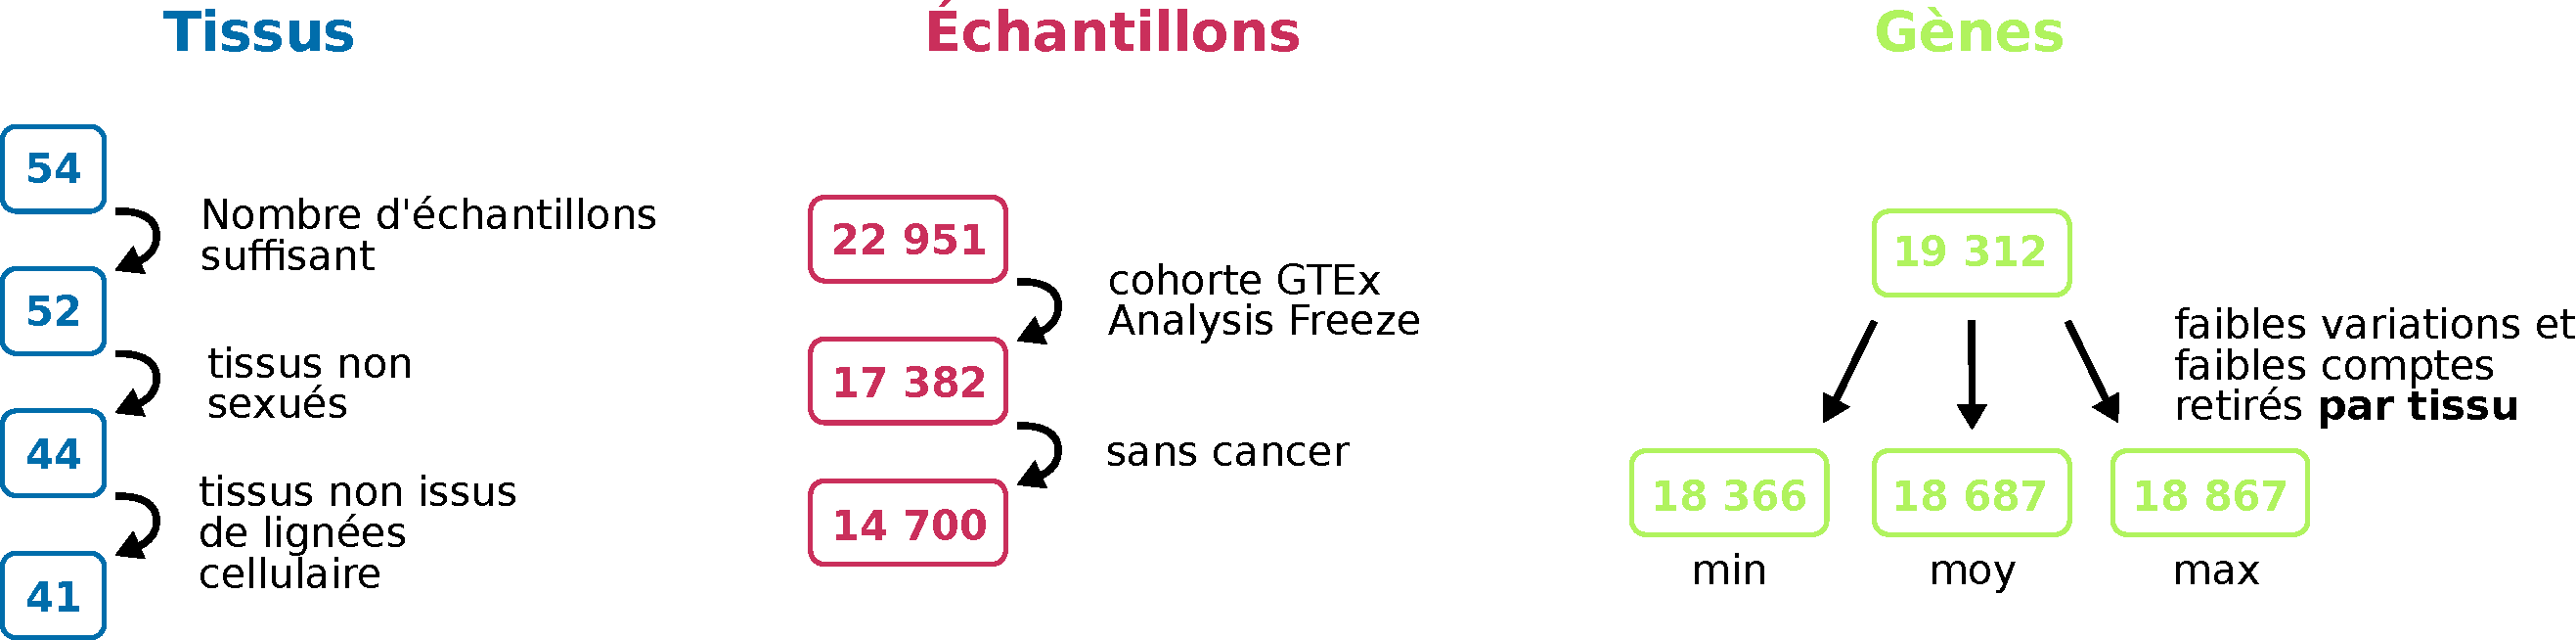
\includegraphics[width=1\textwidth]{img/chap2/chap2_filtre_donnees.pdf}
    % \includesvg[scale=.5]{img/chap2/chap2_filtre_donnees.svg}
    \caption{Ensemble des filtres appliqués sur les différentes données et impact sur les données utilisées pour la construction ultérieure des réseaux de co-expression.}
    \label{figure:data_filters}
    % \caption{Nombre d'échantillons disponibles par tissu et par tranche d'âge de 10 ans dans les données de GTEx.}
\end{figure}


Le vieillissement est un phénomène dont les altérations moléculaires sont linéaires avec le temps, dont les dommages cellulaires sont super-linéaires \citeB{Todhunter2018}, et où la mortalité associée augmente de façon exponentielle passée 20 ans \citeB{Finch2016}. Afin de faciliter la détection de ces altérations grâce à l'analyse de co-expression différentielle, on s'est donc dans un premier temps concentré sur une sélection de tranches d'âges très contrastées. Les échantillons sélectionnés sont issus de donneurs entre 20 et 30 ans pour la tranche qu'on nommera "\textbf{jeune}", et entre 60 et 70 ans pour la tranche qu'on nommera "\textbf{âgée}". Les données de GTEx ne comportent toutefois pas un nombre d'échantillons similaire pour chacune de ces tranches du fait de la mortalité plus importante chez les personnes âgées que les personnes jeunes. Ce déséquilibre est principalement dû aux causes de décès pour chaque tranche d'âge avec des décès par traumatisme chez les jeunes plutôt que par maladie chronique ou maladie liée à l'âge chez les âgés. Un premier filtre de notre pré-traitement restreint donc la sélection des tissus à ceux comportant au minimum 50 échantillons dans chacune des tranches d'âge, ce qui n'est pas le cas de la Vessie (20) et le Rein - Médulla (3). Ce nombre d'échantillons permet d'assurer un bon compromis entre des réseaux de co-expression de gènes robustes, donc non sensibles à des valeurs aberrantes, et la perte de plus de tissus à étudier dans cette analyse multidimensionnelle qu'on souhaite effectuer \citeB{Liesecke2019}.

Tous les tissus restant n'étaient pas nécessairement adaptés à l'étude globale du vieillissement chez l'humain. Ainsi on a retiré tous les tissus liés à un seul sexe : Trompes de Fallope, Col de l'utérus, Utérus, Vagin, Sein, Ovaire, Prostate, Testicule. À ce retrait s'ajoute celui des échantillons de lignées cellulaires (dérivées ou non de tissus eux conservés) car non représentatifs du vieillissement biologique : Cellules - Lymphocytes transformés par EBV, Cellules - Fibroblastes cultivés, Cellules - Lignée cellulaire de leucémie (CML). 


\begin{figure}[ht]
    \centering
    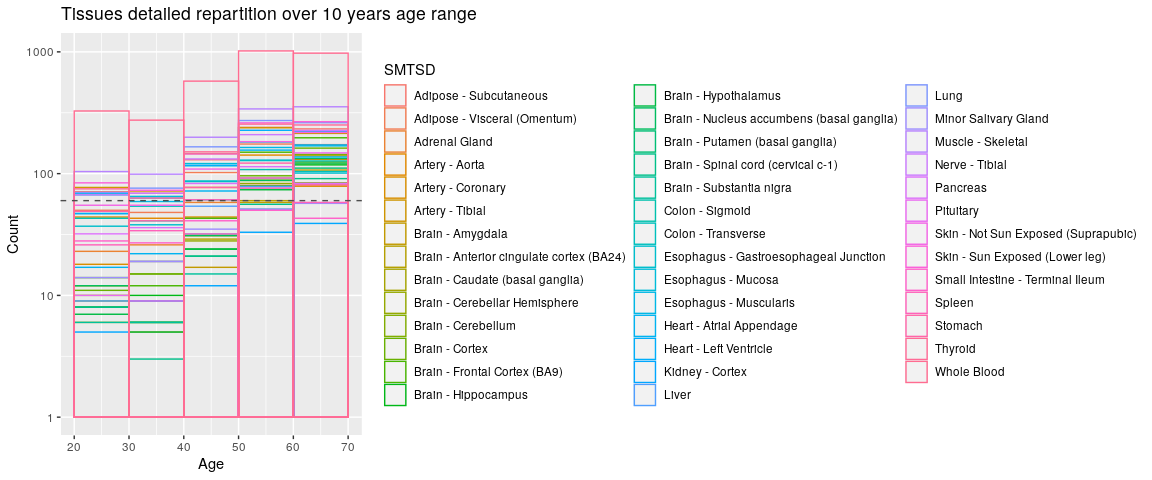
\includegraphics[width=1\textwidth]{img/chap2/chap2_sample_count_by_tissu.png}
    \caption{Nombre d'échantillons disponibles par tissu et par tranche d'âge de 10 ans dans les données de GTEx.}
    \label{figure:sample_count_by_tissu}
\end{figure}


\subsection{Filtre des échantillons}

\begin{figure}[hb]
    \centering
    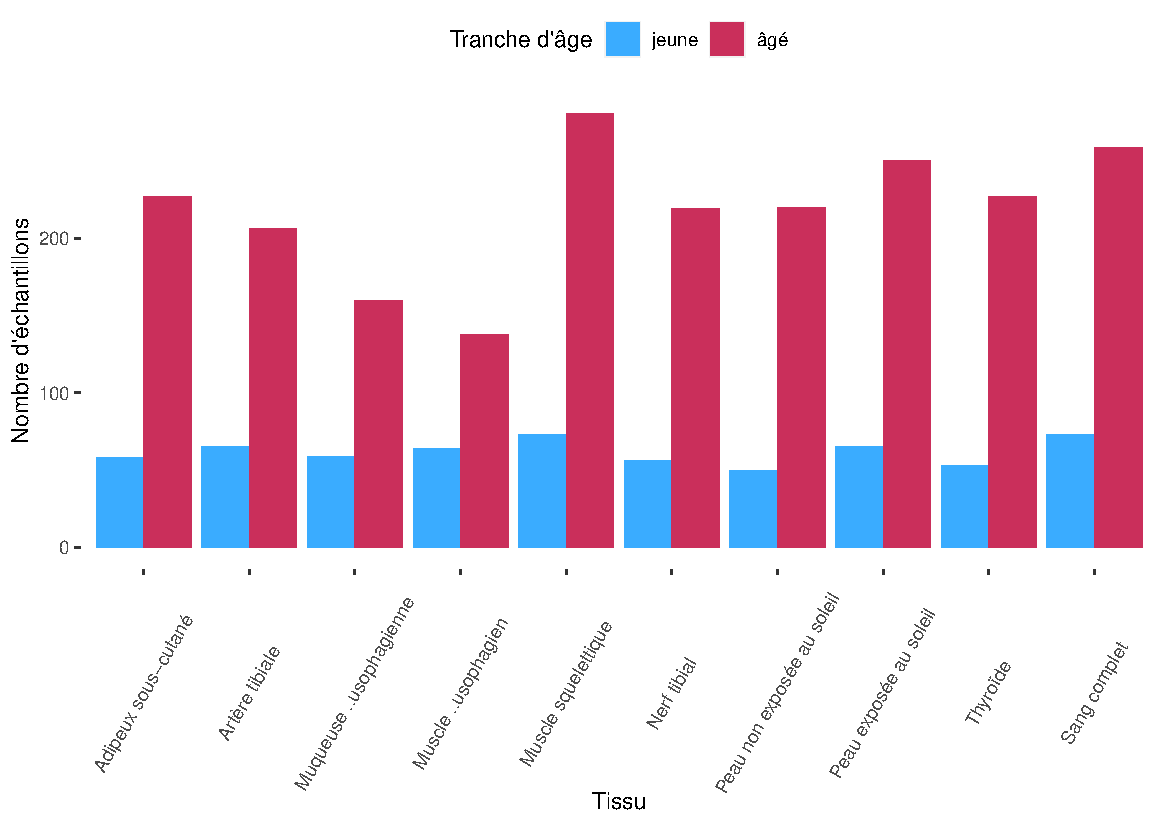
\includegraphics[width=0.8\textwidth]{img/chap2/chap2_sample_count_by_tissu_after_filter.pdf}
    \caption{Nombre d'échantillons disponibles par tissu dans les tranches d'âge jeune (20-30) et âgé (60-70) après filtration selon la cohorte et le statut cancéreux.}
    \label{figure:sample_count_by_tissu_after_filter}
\end{figure}

En plus de ces sélections de tissus, certains échantillons ont directement nécessité une filtration afin de prévenir de potentiels biais qui pourraient altérer l'analyse de co-expression ou l'interprétation des modules en étant issus. Ainsi, seuls les échantillons répondant au critère d'inclusion dans la cohorte "GTEx Analysis Freeze" ont été retenus en premier lieu (Figure \ref{figure:data_filters}. Cette cohorte atteste que les échantillons n'étaient pas :
\begin{itemize}
    \item issus de donneurs ayant des liens de parenté ou de donneurs avec des critères d'exclusion, par exemple des donneurs avec des duplications ou délétions chromosomiques
    \item affectés d'un syndrome tel que défini par la base de données OMIM \citeB{Hamosh2005}, hors maladies liées au vieillissement
    \item ayant effectué une chirurgie de ré-assignation sexuelle
\end{itemize}
% issus de donneurs ayant des liens de parenté ou de donneurs avec des critères d'exclusion, par exemple des donneurs avec des duplications ou délétions chromosomiques, affectés d'un syndrome tel que défini par la base de données OMIM \citeB{Hamosh2005} (ce qui n'inclue pas les maladies liées au vieillissement), ou encore ayant effectué une chirurgie de ré-assignation sexuelle. 

Par ailleurs, l'expression des tissus tumoraux a montré, dans des études préalables, des modèles d'expression génétique différents de ceux non tumoraux \citeB{Tang2017}. Par conséquent, les échantillons de ces donneurs ont également été supprimées ici ainsi que les échantillons dont le statut cancéreux était inconnu. La répartition finale des échantillons par tissu et par tranche d'âge est visible en Figure \ref{figure:sample_count_by_tissu_after_filter}.


\subsection{Filtre sur les gènes}

On a considéré comme base dans cette étude uniquement les gènes codants pour une protéine (d'après GENCODE 26) sur les autosomes. Pour continuer à éviter l'influence du sexe, on a également limité les gènes des gonosomes à ceux du chromosome X. Afin de limiter l'ajout de biais d'origine technique, on a également exclu les gènes dont le compte de lecture (en anglais \textit{count}) était inférieur à 6 dans la totalité des échantillons \citeB{Rocke2001}. Les gènes n'ayant aucune variation se sont vu retirés du jeu de données car leur apport à la co-expression aurait était nul et leur conservation aurait entraîné l'utilisation de ressources inutile. Ces filtres ayant été appliqués par tissu, le nombre de gènes restant varie d'un tissu à un autre avec en moyenne 18687 gènes contre initialement 19 312 (Figure \ref{figure:data_filters}).



\subsection{Correction des facteurs confondants}

À l'instar de l'analyse d'expression différentielle, l'analyse de co-expression différentielle nécessite des données biaisées au minimum pour une construction de réseau de qualité. Ces biais (ou facteurs confondants) peuvent être tant techniques que biologiques et vont entraîner une augmentation de la variation de façon artificielle. Le risque est alors de détecter une différence artificielle et de l'assumer comme expérimentalement pertinente alors qu'elle est en fait due aux biais. Dans le cas de la co-expression plus spécifiquement, ces biais peuvent entraîner des corrélations erronées mais qui semblent crédibles entre certains gènes. Elles altèrent alors la construction du réseau de co-expression et par la suite la détection des modules qui se base sur un découpage en modules via les corrélations. Ainsi, il est essentiel de corriger ces facteurs confondants au préalable de l'utilisation du package R GWENA \citeB{Lemoine2021Dec} sur les données comme on va le faire par la suite.

La complexité de la correction des facteurs confondants réside dans leur suppression sans pour autant altérer la distribution des données ou supprimer le signal expérimental d'intérêt, ici les variations dans le transcriptome dues à l'âge. 
% Il est également important avec l'utilisation de GWENA de veiller à ce que la correction n'altère pas la topologie d'invariance d'échelle qu'on retrouve dans les données de transcriptomique après construction d'un réseau de co-expression \citeB{Zhang2005a}. En effet, cela invaliderait la méthode de détection des modules ultérieure car celle-ci repose sur une méthode présupposant la présence d'une telle topologie pour fonctionner.
Il est également important avec l'utilisation de GWENA de veiller à ce que la correction n'altère pas la topologie d'invariance d'échelle (\textit{scale-free topology}) qu'on retrouve dans les réseaux de co-expression construits sur des données de transcriptomique \citeB{Zhang2005a}. Cette propriété assure que la distribution des degrés des nœuds suivent en fait une loi de puissance. Briser cette topologie perturberait la détection des modules dans le réseau car la méthode employée pour cela présuppose la présence d'une telle topologie pour fonctionner.

% \todo{Je me demande si ces 2 paragraphes plus haut ne devraient pas finir en intro de thèse}

% La base de données GTEx n'échappe pas aux biais \citeB{Parsana2019} et a même été étudiée sur le plan de la contamination \citeB{Nieuwenhuis2020}.
La base de données GTEx n'échappe pas aux biais \citeB{Parsana2019, Nieuwenhuis2020} et doit donc passer par cette étape sensible de correction des facteurs confondants dans le cadre de notre analyse de co-expression.
Malgré le progrès de techniques ciblées sur des facteurs confondants connus comme l'effet de lot, l'effet de centre de prélèvement, le sexe, le poids, etc., celles-ci ne sont pas capables de corriger pour des facteurs peu explicites ou diffus comme la classe sociale, l'alimentation, la façon de manipuler des techniciens, etc. La correction par composante principale (CP) vise à répondre à ce type de problématique et a montré de bons résultats selon une évaluation par validation de voies de signalisation au sain de modules détectés \citeB{Parsana2019}. Elle a également montré de meilleurs résultats que d'autres méthodes telles que la régression multiple, le taux exonique, ou encore le numéro d'intégrité d'ARN (\textit{RNA integrity number}, ou RIN). Fait important pour la co-expression en particulier, cette méthode conserve la propriété d'invariance d'échelle des données requise pour la construction des modules de co-expression dans notre méthode.


\begin{table}[h!]
\centering
\begin{tabular}{llll}
\multirow{2}{*}{\textbf{Tissu}} & \multirow{2}{*}{\textbf{\begin{tabular}[c]{@{}l@{}}Nombre de CP \\ corrigées\end{tabular}}} & \multicolumn{2}{l}{\textbf{Nombre d'échantillons}} \\ \cline{3-4} 
                                &                                                                                             & \textbf{Jeune}            & \textbf{Âgé}           \\ \hline
Adipeux sous-cutané             & 1                                                                                           & 58                        & 227                    \\
Artère tibiale                  & 3                                                                                           & 65                        & 206                    \\
Muqueuse œusophagienne          & 1                                                                                           & 59                        & 160                    \\
Muscle œusophagien              & 3                                                                                           & 64                        & 138                    \\
Muscle squelettique             & 5                                                                                           & 73                        & 281                    \\
Nerf tibial                     & 4                                                                                           & 56                        & 219                    \\
Peau non exposée au soleil      & 4                                                                                           & 50                        & 220                    \\
Peau exposée au soleil          & 3                                                                                           & 65                        & 250                    \\
Thyroïde                        & 3                                                                                           & 53                        & 227                    \\
Sang complet                    & 1                                                                                           & 73                        & 259                   
\end{tabular}
\caption{Résumé du nombre de composantes utilisées pour effectuer la correction de l'expression par tissu, ainsi que le nombre d'échantillons inclus dans chacun pour les deux tranches d'âge.}
\label{table:nb_PC_corr_and_samples_by_tissue}
\end{table}


Cependant, cette correction va également corriger l'âge qui est notre variable d'intérêt. Afin de conserver cette information tout en ayant un effet de correction par CP sur les autres facteurs confondants, on a donc ajusté la méthode estimant le nombre $n$ de CP par lequel corriger les jeux de données. Au lieu d'utiliser une procédure de permutation \citeB{Buja1992Oct}, l'estimation de $n$ s'est faite en deux étapes :
\begin{itemize}
    \item Un test de corrélation de chaque gène avec l'âge associé à chaque échantillon (donc patient) en fonction de différent $n$ PC corrigées donne une liste de gènes significativement associés à l'âge.
    \item Cette liste de gènes par $n$ PC corrigées est ensuite croisée avec deux bases de données de gènes connus comme étant associés au vieillissement : GenAge \citeB{DeMagalhaes2004} et Digital Aging Atlas \citeB{Craig2015}. Y sont alors compté le nombre de gènes significatifs recoupés.
\end{itemize}
Finalement, le $n$ de PC à corriger retenu est celui où le nombre de gènes significatifs est le plus haut dans chaque base de données. En cas de divergence de ce $n$ entre les bases de données, on a sélectionné la valeur la plus basse de $n$ afin de ne pas risquer de corriger l'âge (Table \ref{table:nb_PC_corr_and_samples_by_tissue}).


% \todo[inline]{Idée de figure : remplacer cette table ou en touts cas la partie nb composantes par un ensemble de mini histogrames avec les deux bdd en un, et en facet pour chaque tissu.}


\subsection{Construction du réseau, détection des modules et co-expression différentielle}

Une fois les données pré-traitée, nous avons généré un réseau de co-expression de gènes indépendamment sur chacun des 10 tissus et tranche d'âge à l'aide du package GWENA \citeB{Lemoine2021Dec}. Les paramètres spécifiés étaient ceux par défaut de la fonction \verb+build_net+ à l'exception de la corrélation qui était basée sur Spearman et du seuil d'ajustement de la loi de puissance fixé à 0,8. Dans chaque réseau de tissu, on a ensuite détecté le nombre de modules via la fonction \verb+detect_modules+ selon un seuil de coupe de l'arbre hiérarchique identique dans chaque tissu et une taille de module minimale fixée à 20 gènes. Chaque ensemble de modules a ensuite été testé à l'aide de la fonction \verb+compare_conditions+ par tissu entre les deux tranches d'âges pour identifier les modules préservés, modérément préservés et non préservés avec le vieillissement.

\subsection{Investigation des phénomènes communs ou spécifiques du vieillissement}

\begin{figure}[hb]
    \centering
    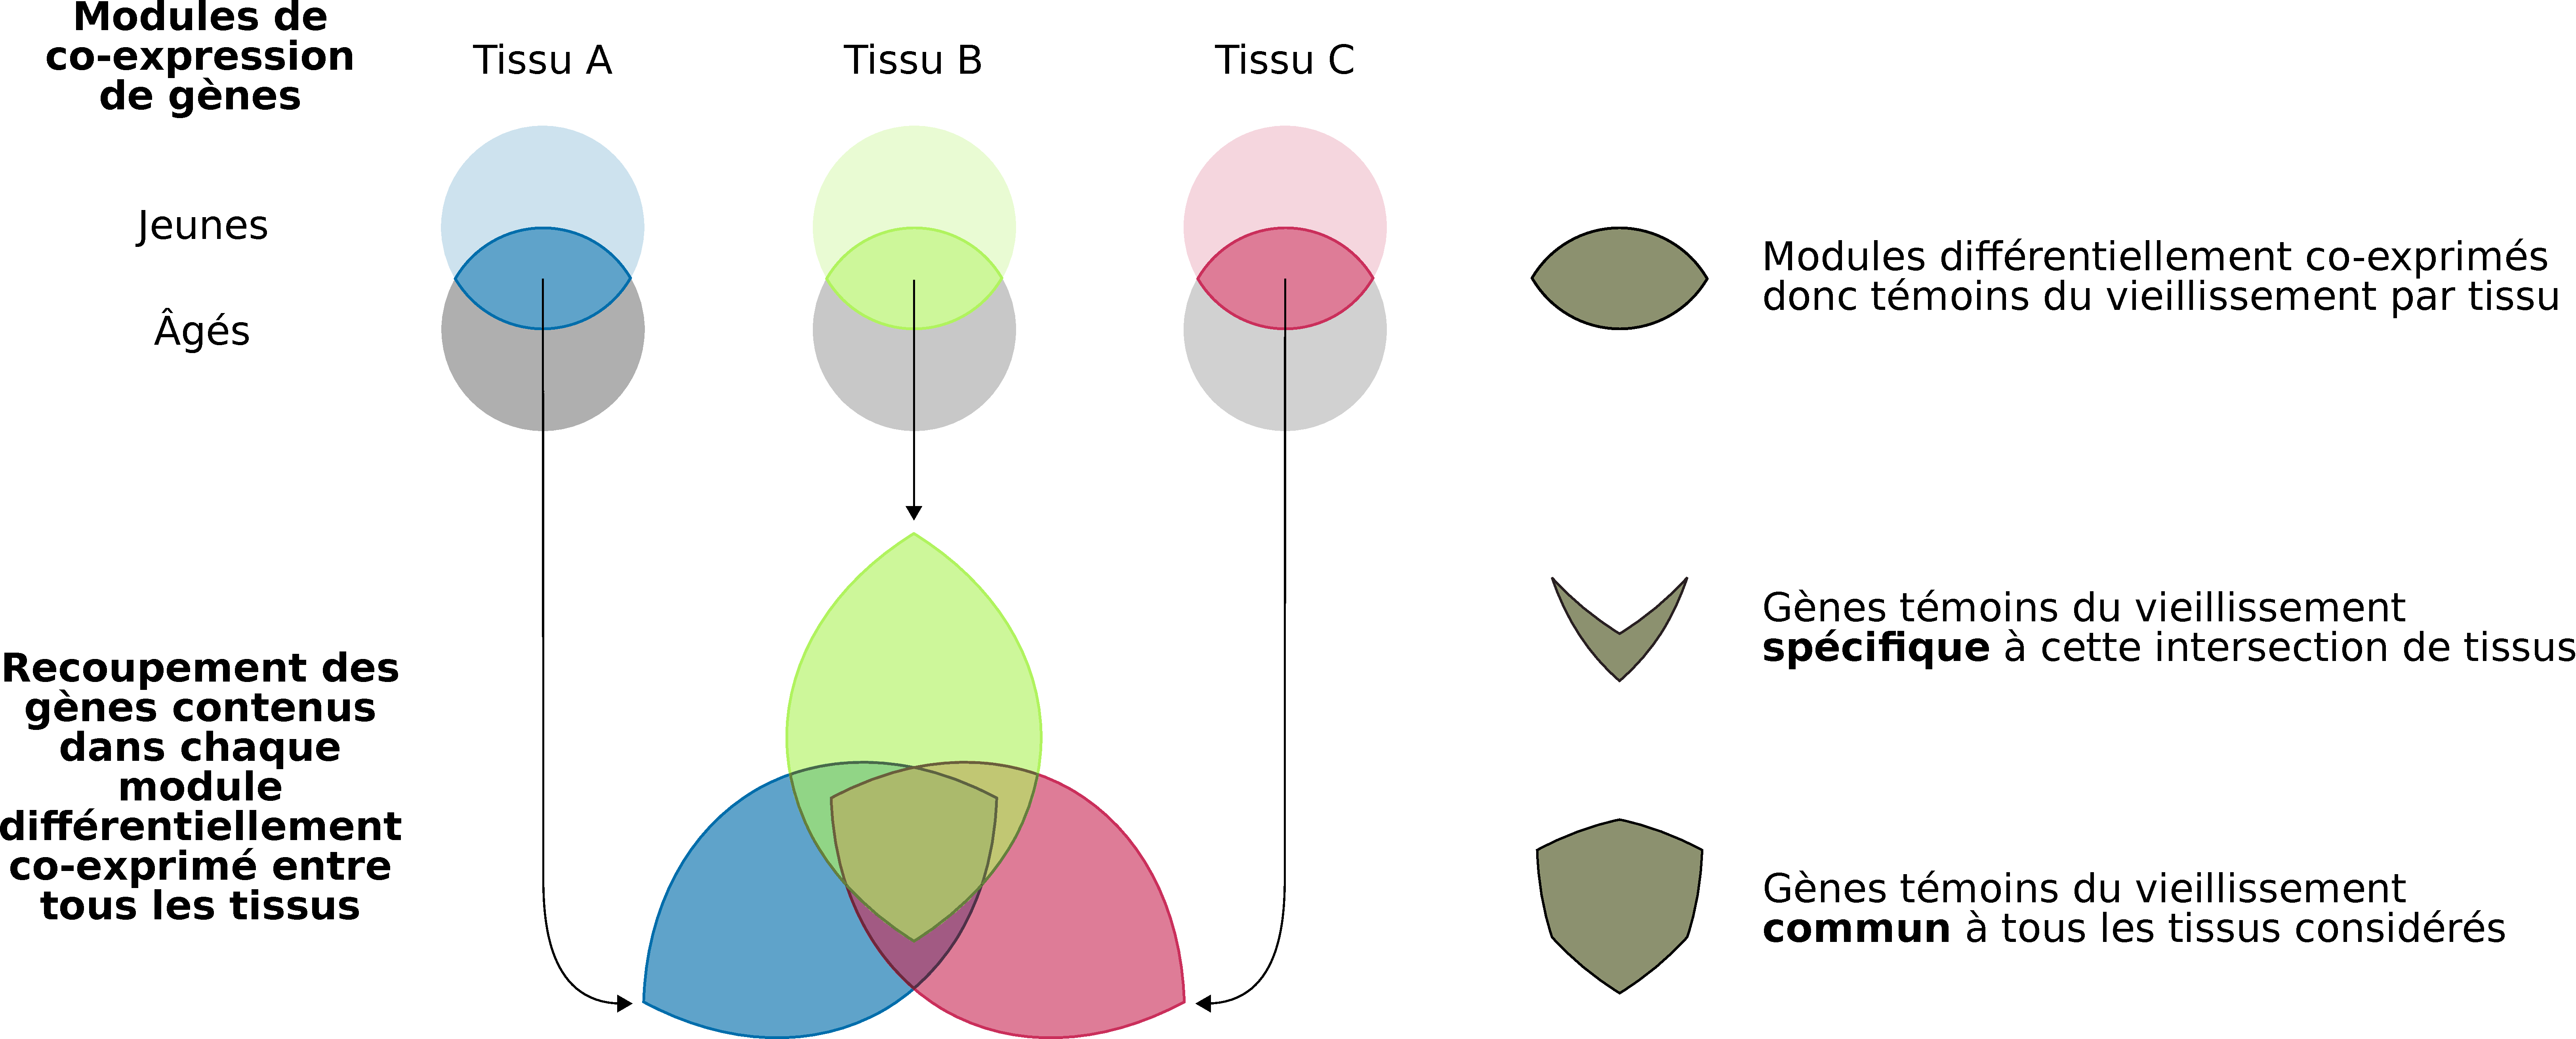
\includegraphics[width=1\textwidth]{img/chap2/chap2_intersection_explication.pdf}
    \caption{Schéma simplifié, avec trois tissus seulement, de la méthode de construction des intersections spécifiques et communes du vieillissement.}
    \label{figure:chap2_intersection_explication}
\end{figure}

Dans chaque tissu on a isolé les modules de co-expression modérément préservés (MP) et non préservés (NP) entre les deux tranches d'âge. On a ensuite effectué une intersection de leur contenu en gènes entre tous les tissus afin d'isoler les gènes participant à des phénomènes communs à plusieurs tissus et ceux participant à des phénomènes plus spécifiques d'un sous ensemble de tissus partageant des propriétés biologiques \ref{figure:chap2_intersection_explication}. Tous ont ensuite été enrichis via la fonction \verb+bio_enrich+ de GWENA et leurs résultats revus en regard de la littérature sur le vieillissement. Pour les plus pertinents d'entre eux, un résumé des termes Gene Ontology selon leur similarité sémantique a été réalisé à l'aide du package R rrvgo \citeB{rrvgo2021} qui reprend le principe de l'outil REVIGO \citeB{Supek2011Jul}.



\section{Résultats}

\subsection{Répartition des gènes en fonction de la tranche d'âge et du tissu}

\begin{figure}[!hb]
    \centering
    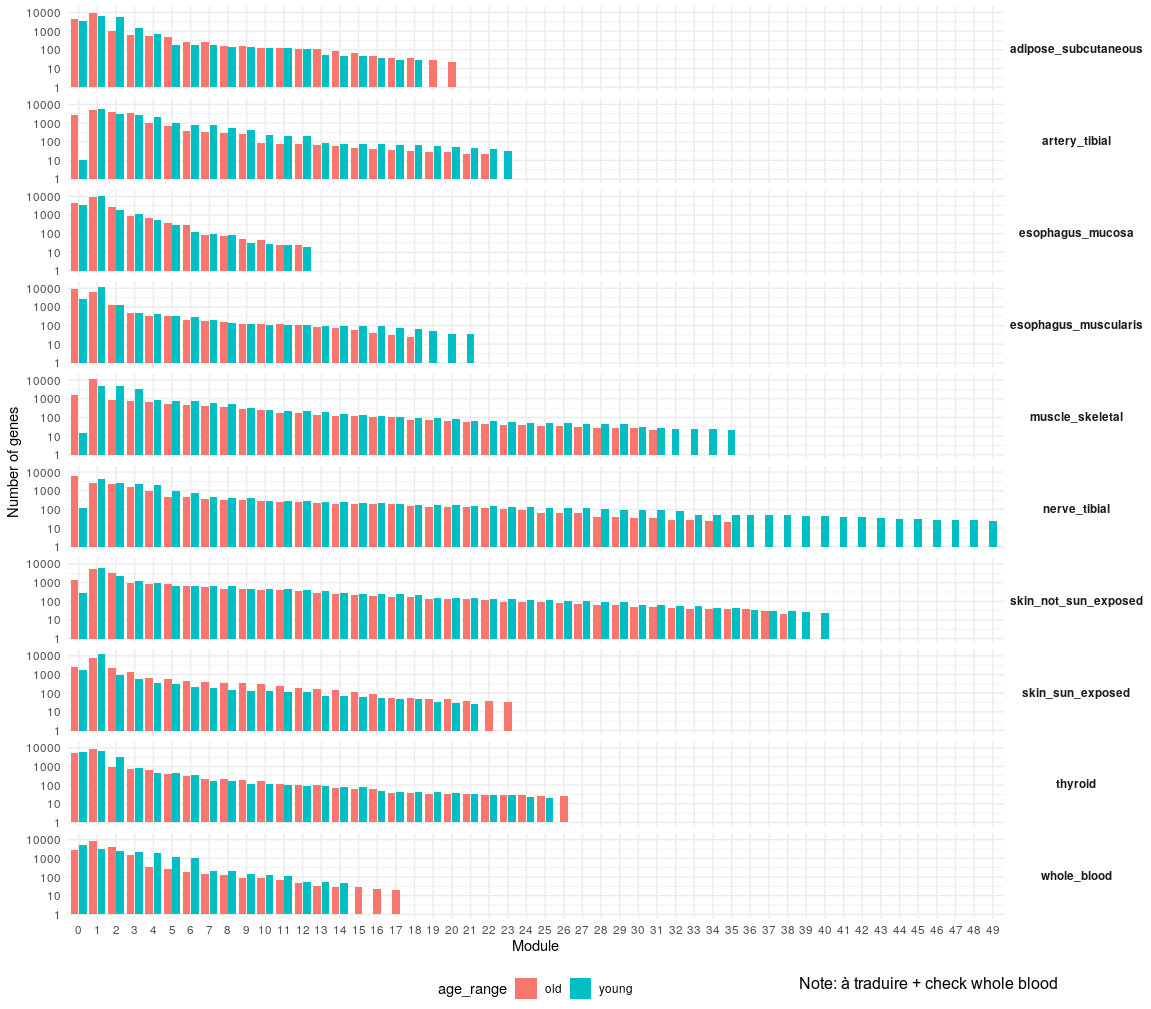
\includegraphics[width=0.95\textwidth]{img/chap2/chap2_repartition_genes_modules_tissus.png}
    \caption{Répartition des gènes (en échelle log10) pour chaque tissu entre les deux tranches d'âge jeune (bleu) et âgée (rouge)}
    \label{figure:repartition_genes_modules_tissus}
\end{figure}

La répartition des gènes entre les modules est hétérogène, tant entre les tranches d'âge qu'entre les tissus (Figure \ref{figure:repartition_genes_modules_tissus}), avec une moyenne à 26 modules tout confondu (25.2 pour les âgés et 26.8 pour les jeunes). Le module 0 présent sur la figure regroupe les gènes sans association à un module. Celui-ci est quasi systématiquement plus grand dans la tranche âgée que jeune, à l'exception des tissus de la thyroïde et du sang complet. Les tissus où cet écart est le plus creusé sont ceux disposant du plus grand nombre de modules dans la tranche d'âge jeune. Ces résultats sont cohérents avec la tendance à la perte de co-expression constatée dans les tranches d'âge âgées \citeB{Southworth2009} : la perturbation des voies de signalisation au cours du vieillissement entraîne une diminution de la co-expression entre gènes de ces voies.


\subsection{Modules spécifiques du vieillissement et recoupement inter-tissus}

Le but étant de rechercher des origines communes au vieillissement entre tous les tissus, on a ensuite effectué une étape de co-expression différentielle intra tissu. La tranche d'âge jeune a été prise pour référence, c’est-à-dire que le test indiquera si chaque module détecté dans la tranche d'âge jeune est préservé, modérément préservé, non préservé, ou non concluant. Les résultats ont été résumés en Table \ref{table:modules_status_all_tissues}. 

On y constate que certains tissus tendent à avoir proportionnellement moins de modules préservés lors du vieillissement. Avec moins de 50 \% de préservation on retrouve notamment le muscle œsophagien et squelettique, ainsi que de la peau exposée au soleil et la thyroïde. À cela s'ajoute que la peau exposée au soleil et le muscle squelettique sont les deux tissus ayant le plus de modules non préservés proportionnellement à leur nombre de modules.

\begin{table}[!ht]
\resizebox{\textwidth}{!}{
\begin{tabular}{llllllllll}
\multirow{2}{*}{\textbf{Tissu}} & \multicolumn{2}{l}{\textbf{Préservé}} & \multicolumn{2}{l}{\textbf{Modérement préservé}} & \multicolumn{2}{l}{\textbf{Non préservé}} & \multicolumn{2}{l}{\textbf{Non concluant}} & \textbf{Total} \\ \cline{2-10} 
                                & \textbf{\#}       & \textbf{\%}       & \textbf{\#}             & \textbf{\%}            & \textbf{\#}         & \textbf{\%}         & \textbf{\#}          & \textbf{\%}         & \textbf{\#}    \\ \hline
Adipeux sous-cutané             & 12                & 67              & 4                       & 22                   & 0                   & 0                 & 2                    & 11               & 18             \\
Artère tibiale                  & 13                & 57              & 8                       & 35                   & 1                   & 4                 & 1                    & 4                & 23             \\
Muqueuse œusophagienne          & 3                 & 25              & 8                       & 67                   & 1                   & 8                 & 0                    & 0                & 12             \\
Muscle œusophagien              & 9                 & 43              & 6                       & 29                   & 0                   & 0                 & 6                    & 29               & 21             \\
Muscle squelettique             & 14                & 40              & 13                      & 37                   & 5                   & 14                & 3                    & 9                & 35             \\
Nerf tibial                     & 35                & 71              & 9                       & 18                   & 1                   & 2                 & 4                    & 8                & 49             \\
Peau non exposée au soleil      & 36                & 90              & 4                       & 10                   & 0                   & 0                 & 0                    & 0                & 40             \\
Peau exposée au soleil          & 10                & 48              & 8                       & 38                   & 2                   & 10                & 1                    & 5                & 21             \\
Thyroïde                        & 12                & 48              & 8                       & 32                   & 1                   & 4                 & 4                    & 16               & 25             \\
Sang complet                    & 9                 & 64              & 4                       & 29                   & 0                   & 0                 & 1                    & 7                & 14              
\end{tabular}
}
\caption{Nombre (\#) et ratio (\%) de modules par statut de préservation selon chaque tissu.}
\label{table:modules_status_all_tissues}
\end{table}


Afin d'observer des similarités de mécanismes du vieillissement entre ces différents tissus, on a dans un premier temps regardé si des gènes communs existaient entre les modules modérément préservés (MP) et non  préservés (NP). Le diagramme UpSet \citeB{Lex2014} visible en Figure \ref{figure:upset_intersection_genes_tissu_unpres_modpres} permet de constater le faible recouvrement entre les gènes contenus dans les modules MP et NP. Ce diagramme révèle également que le maximum de tissus avec des gènes communs est 5. Ce chiffre est à mettre en contraste avec le fait que les modules créés par GWENA pour un même tissu ne sont pas chevauchant. Un gène classé dans un module ne sera donc pas également classé dans un autre et on aurait pu espérer une intersection au maximum de taille 10 étant donné qu'on dispose de 10 tissus. 

\begin{landscape}
\begin{figure}[p]
  \centering
  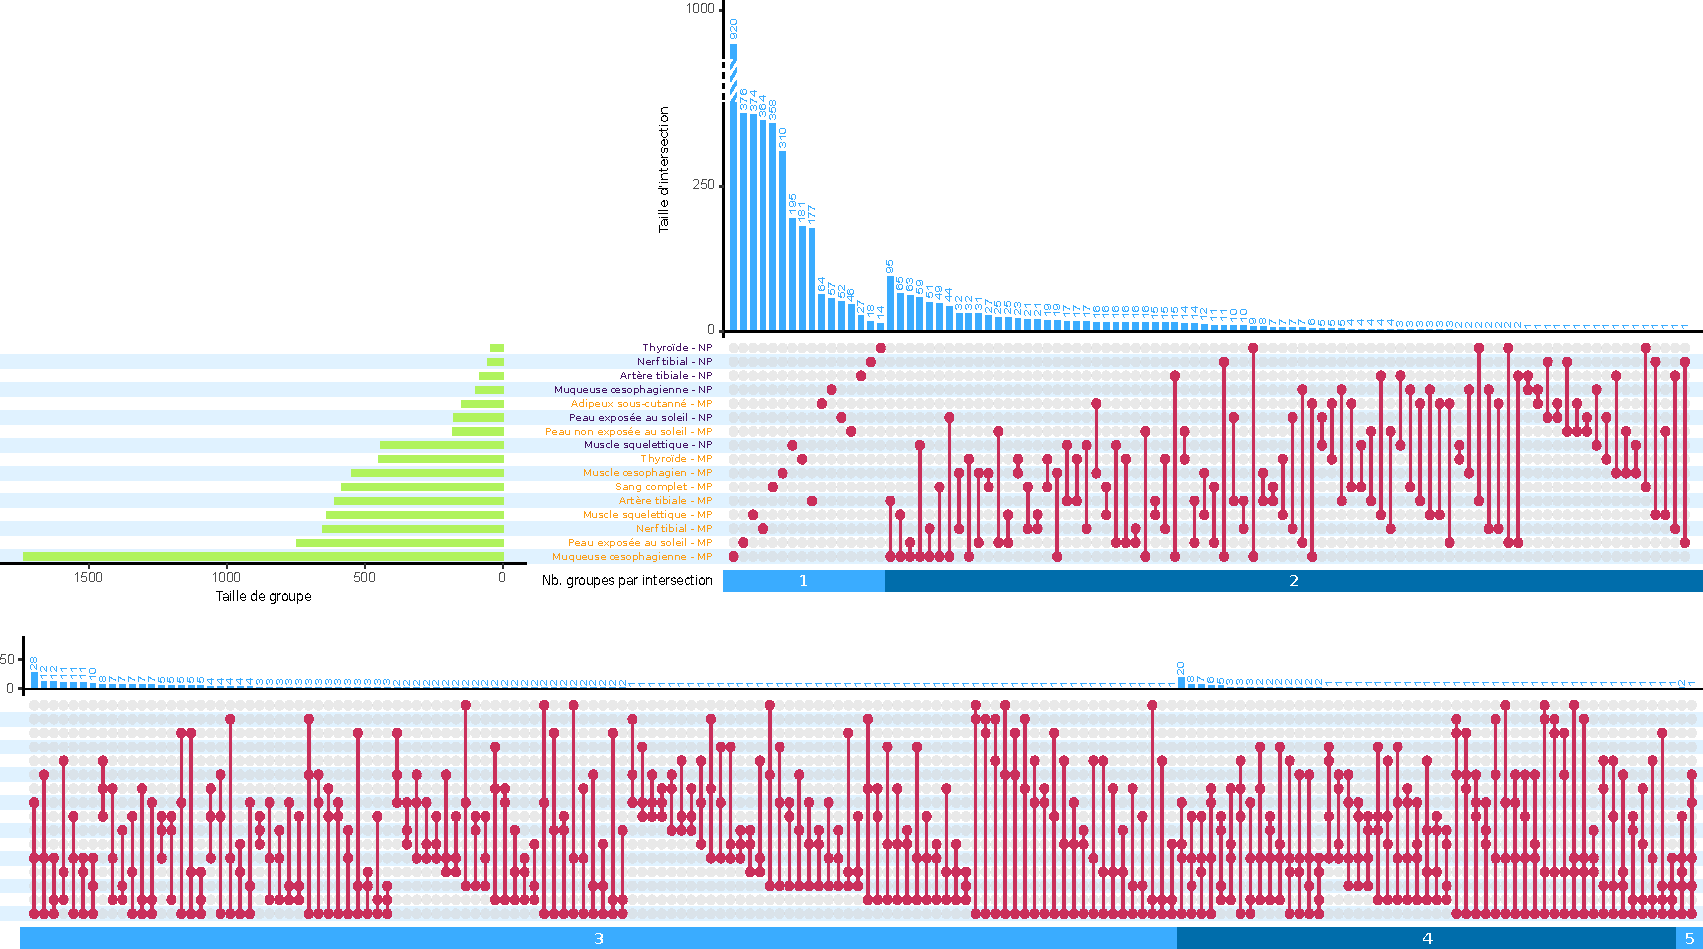
\includegraphics[width=1.5\textheight]{img/chap2/chap2_upset_genes_unpres_modpres_by_tissue.pdf}
  \caption[Intersections entre tous les jeux de gènes pour chaque couple tissu / statut de préservation]{Intersections entre tous les jeux de gènes pour chaque couple tissu / statut de préservation. Le diagramme Upset est une représentation qui vise à remplacer une visualisation par diagramme de Venn, ce dernier n'étant pas adaptée à la représentation de plus de 5 catégories. La matrice d'intersection (en orange) indique quel couple tissu / statut est considéré dans l'intersection (rose si pris en compte, gris si non) et quels sont les autres tissus dans cette intersection (ligne rose). L'histogramme des tailles de groupe (gris) à gauche de la matrice indique le nombre total de gène contenu dans le couple tissu / statut en ligne. L'histogramme des tailles d'intersection indique le nombre de gènes contenu dans l'intersection indiquée en matrice d'intersection pour cette colonne.}
  \label{figure:upset_intersection_genes_tissu_unpres_modpres}
\end{figure}
\end{landscape}

En plus de ce nombre maximal de tissus présent dans une intersection, certains tissus vont se retrouver plus fréquemment dans ces intersections en raison de leur nombre de modules MP/NP ou de modules contenant plus de gènes (Table \ref{table:modules_status_all_tissues}). Ainsi, les modules MP de la muqueuse œsophagienne regroupent 1750 gènes et tendent à se positionner dans plus d'intersection que la moyenne. Une séparation est toutefois visible entre les deux types de statut MP et NP dans les intersections au-delà de 2 tissus et avec un minimum de trois gènes.


\subsection{Répartition des phénomènes communs liés au vieillissement dans plusieurs tissus}

\begin{table}[hb]
\centering
\resizebox{0.8\textwidth}{!}{
\begin{tabular}{@{}lllllllllll@{}}
\rotatebox{90}{\textbf{Muqueuse œusophagienne}}   & \rotatebox{90}{\textbf{Artère tibiale}}                      & \rotatebox{90}{\textbf{Thyroïde}}                 & \rotatebox{90}{\textbf{Muscle squelettique}}      & \rotatebox{90}{\textbf{Peau exposée au soleil}}   & \rotatebox{90}{\textbf{Muscle œusophagien}}       & \rotatebox{90}{\textbf{Nerf tibial}}              & \rotatebox{90}{\textbf{Peau non exposée au soleil}} & \rotatebox{90}{\textbf{Adipeux sous-cutané}}      & \rotatebox{90}{\textbf{Sang complet}}             & \textbf{Phénomène du vieillissement observé}       \\ \midrule
\cellcolor[HTML]{F8A102} & \cellcolor[HTML]{F8A102}            &                          & \cellcolor[HTML]{F8A102} &                          &                          &                          & \cellcolor[HTML]{F8A102}   &                          &                          & Homéostasie                               \\
                         & \cellcolor[HTML]{F8A102}            & \cellcolor[HTML]{F8A102} &                          &                          & \cellcolor[HTML]{F8A102} &                          &                            &                          &                          & Régulation de la transcription            \\
\cellcolor[HTML]{F8A102} &                                     & \cellcolor[HTML]{F8A102} & \cellcolor[HTML]{F8A102} &                          &                          &                          &                            &                          &                          & Dérivés réactifs de l'oxygène - peroxydes \\
                         &                                     & \cellcolor[HTML]{F8A102} &                          & \cellcolor[HTML]{F8A102} & \cellcolor[HTML]{F8A102} & \cellcolor[HTML]{F8A102} &                            &                          &                          & Dérivés réactifs de l'oxygène - dGTP      \\
                         &                                     & \cellcolor[HTML]{F8A102} &                          &                          &                          &                          & \cellcolor[HTML]{F8A102}   & \cellcolor[HTML]{F8A102} &                          & Inflammation                              \\
                         &                                     &                          &                          & \cellcolor[HTML]{F8A102} & \cellcolor[HTML]{F8A102} & \cellcolor[HTML]{F8A102} &                            &                          &                          & Désamination                              \\
\cellcolor[HTML]{F8A102} & \cellcolor[HTML]{F8A102}            &                          &                          &                          &                          & \cellcolor[HTML]{F8A102} &                            &                          &                          & Coagulation - plaquettes                  \\
\cellcolor[HTML]{F8A102} & \cellcolor[HTML]{F8A102}            & \cellcolor[HTML]{F8A102} &                          &                          &                          & \cellcolor[HTML]{F8A102} &                            &                          &                          & Coagulation - global                      \\
\cellcolor[HTML]{F8A102} & \cellcolor[HTML]{F8A102}            &                          & \cellcolor[HTML]{F8A102} &                          &                          &                          &                            &                          &                          & Méthylation - folate, B12, selenium       \\
                         &                                     &                          & \cellcolor[HTML]{F8A102} & \cellcolor[HTML]{F8A102} &                          &                          &                            & \cellcolor[HTML]{F8A102} &                          & Méthylation - déméthylase                 \\
\cellcolor[HTML]{F8A102} & \cellcolor[HTML]{F8A102}            &                          & \cellcolor[HTML]{F8A102} &                          &                          &                          &                            &                          & \cellcolor[HTML]{F8A102} & Altération de la MEC                      \\
                         &                                     & \cellcolor[HTML]{F8A102} &                          & \cellcolor[HTML]{F8A102} & \cellcolor[HTML]{F8A102} &                          &                            &                          &                          & Anomalie du taux de glutamine             \\
\cellcolor[HTML]{F8A102} &                                     &                          &                          & \cellcolor[HTML]{F8A102} &                          &                          & \cellcolor[HTML]{F8A102}   &                          &                          & Synthèse de pigment (dont mélanine)      \\
\cellcolor[HTML]{F8A102} & \cellcolor[HTML]{F8A102}            & \cellcolor[HTML]{F8A102} & \cellcolor[HTML]{F8A102} &                          &                          &                          &                            &                          &                          & Anomalie du taux de fer                   \\
\midrule
8                        & 7                                   & 7                        & 6                        & 5                        & 4                        & 4                        & 3                          & 2                        & 1                        & \textbf{Total}                   
\end{tabular}
}
\caption[Phénomènes connus dans le vieillissement et observés dans les intersections de modules MP et NP pour chaque tissu]{Phénomènes connus dans le vieillissement et observés dans les intersections de modules MP et NP pour chaque tissu. Les modules MP et NP ont été joints par tissus et les tissus ont été ordonnés par nombre décroissant de phénomènes du vieillissement présent. MEC : Matrice extra-cellulaire.}
\label{table:intersection_aging_global_phenomenons}
\end{table}


Pour mieux comprendre les fonctions physiologiques communes en jeu et pouvant être impliquées dans le vieillissement, les intersections de plus de 3 tissus et ayant au moins 5 gènes ont été enrichies via GWENA. Comme visible en Annexe \ref{annexe:chap_2_genes_intersect_enrichments} dans les tables des enrichissements obtenus, 5 intersections n'ont pas donné d'enrichissement significatif malgré un nombre de gènes équivalent à d'autres intersections avec enrichissement. Les 18 autres intersections ont quant à elles retourné des fonctions physiologiques (Gene Ontology \citeB{Ashburner2000}, CORUM \citeB{Ruepp2008}) et voies d'activation (KEGG \citeB{Kanehisa2019}, REACTOME \citeB{Fabregat2016}, WikiPathways\citeB{Slenter2018}) connues comme faisant partie du vieillissement global, ou de manifestations spécifiques à plusieurs tissus. Ainsi on retrouve, dans ces intersections de modules peu ou pas préservés dans la tranche âgée, des fonctions associées à l'homéostasie, la régulation de la transcription, la gestion des dérivés réactifs de l'oxygène, l'inflammation, etc. (Table \ref{table:intersection_aging_global_phenomenons} et Figure \ref{figure:revigo_resume_4_enrich}). La muqueuse œsophagienne bien qu'ayant un nombre de gènes plus élevé que les autres tissus ne se retrouve pas sur-représentée dans ces phénomènes observés. Cela indique donc que la majorité de ses gènes se trouvent dans les intersections de faible taille, tant en gènes qu'en nombre de tissus recoupés. Le sang complet, le tissu adipeux sous-cutané et la peau non exposée au soleil sont eux les tissus les moins présents dans ces intersections avec des phénomènes liés au vieillissement. Le sang complet est notablement absent des intersections avec des phénomènes liés à la coagulation. Les tissus ayant un fort renouvellement (voir en Table \ref{table:tissu_telomere_effet}) que sont les épithéliums (peau exposée au soleil, artère tibiale, muqueuse œsophagienne) sont porteurs d'un grand nombre de phénomènes, ainsi que la thyroïde et le muscle squelettique. 


\begin{figure}[ht]
    \centering
    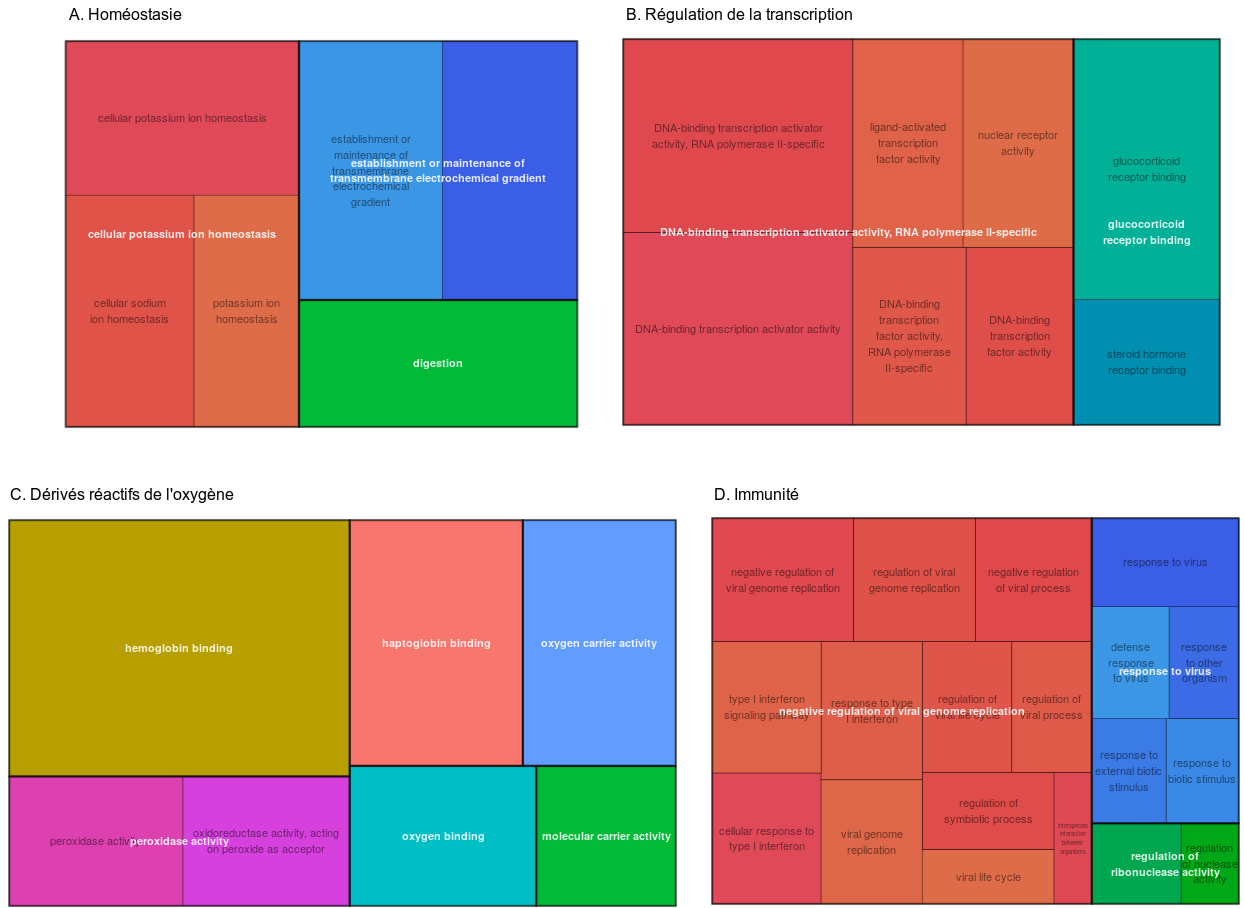
\includegraphics[width=1\textwidth]{img/chap2/chap2_revigo_resume_4_enrich.png}
    \caption[Exemple de résumé des enrichissements sur GO pour 4 des intersections par carte proportionnelle]{Exemple de résumé des enrichissements sur GO pour 4 des intersections par carte proportionnelle. Chaque ensemble de GO terme partageant une ontologie parente commune (selon un score de similarité) est groupé sous une même couleur. Chaque carte présente ici un phénomène connu dans le vieillissement : A. Homéostasie (GO \textit{Biological Process}), B. Régulation de la transcription (GO \textit{Biological Process}), C. Dérivés réactifs de l'oxygène (GO \textit{Molecular Function}), D. Inflammation (GO \textit{Biological Process}) }
    \label{figure:revigo_resume_4_enrich}
\end{figure}

Des anomalies phénotypiques ont été relevées (via enrichissement sur HPO \citeB{Kohler2019}) et présentent un lien parfois direct avec les altérations physiologiques précédemment relevées, et parfois plus éloigné car issues d'une chaine d'événements et réactions physiologiques. 
À ces anomalies du taux de fer détectés dans les fonctions physiologiques coïncident ainsi des phénotypes d'anémie (déficience en taux de globules rouges ou en concentration d'hémoglobine) ou de défaut de coagulation avec hémorragies diverses (épistaxis, saignement gingival, menstruations hors cycle, hémorragie cérébrale). De même, les tissus présentant une altération de la matrice extra-cellulaire (MEC) ont été associés avec des taux élevés de protéine C-réactive et d'anomalies de la fonction exocrine du pancréas ainsi que de malabsorption des lipides et ce qui en découle (stéatorrhée, pancréatite, thrombose veineuse). Ces résultats confirment le lien entre vieillissement et dérèglement progressif de l'homéostasie entrainant en cascade des pathologies de trouble de la coagulation \citeB{Franchini2006,Kario1993} et de la dégradation des lipides circulants \citeB{Yamamoto2014, Hirschfield2003}. Cependant d'autres résultats semblent moins intuitifs comme dans le cas de pathologies liées au sexe (azoospermie, maladie d'hérédité gonosomale) relevées parallèlement à la déméthylation dans le tissu adipeux, le muscle squelettique et la peau non exposée au soleil. Ces informations, en l'absence d'erreur technique, semblent continuer de montrer la complexité des relations entre pathologies et vieillissement.

Enfin, on a exploré le vieillissement et son phénomène de perturbation de la régulation de la transcription en évaluant l'enrichissement d'éléments de régulation (MiRTarBase \citeB{Chou2018}, TRANSFAC \citeB{Matys2006}). L'intersection présentant des phénomènes de coagulation globale est ainsi fortement enrichi en micro ARN (miARN). Ceux-ci contiennent notamment des miARN associés aux 3 gènes de la génération de fibrinogène FGA, FGB, FGG comme détectés lors du chapitre précédent. Quelques autres intersections. Deux facteurs de transcription (FT), HNF1A et HNF1B, sont également significatifs bien que normalement exprimés dans le foie. Cela s'explique par la production de facteurs de la coagulation (dont FGA, FGB, FGG) dans celui-ci et un effet connu de l'altération de production de ces facteurs dans le cadre d'une perturbation de l'expression de HNF1A et HNF1B \citeB{Costa2003}. L'intersection associée à l'inflammation quant à elle ne présente qu'un seul miARN agissant ici sur RSAD2, IFI44, OASL, et EPSTI1 présents dans l'intersection. RSAD2 et OASL sont également connus pour être stimulé par des interférons de type I (\textalpha{} et \textbeta{}) qui ont entre autres IRF1 (pour \textit{interferon related factor 1}) pour FT \citeB{Schoggins2011}. Ce facteur IRF1 fait par ailleurs parti de la liste des FT détectés dans cette intersection. On y trouve un large panel d'autres membres de la famille d'IRF (de 1 à 9 à l'exception d'IRF6) dont l'implication dans l'inflammation s'exerce tant dans la réaction innée qu’acquise \citeB{Frisch2020}. Mais tous les FT détectés via enrichissement n'étaient pas des IRF. Bien que n'étant pas directement liés à la régulation des interférons, STAT2 est présent dans la voie de signalisation des interférons \textalpha{} et \textbeta{} détecté plus tôt (R-HSA-909733). Le dernier FT identifié, FOXP1, n'est quant à lui pas contenu dans cette voie, mais agit sur l'engagement des cellules souches mésenchymateuses et la sénescence au cours du vieillissement \citeB{Infante2018} et sur de la régulation d'autres cytokines, l'interleukine 1 et 12 d'après UniprotKB (Q9H334).

\begin{figure}[p]
    \centering
    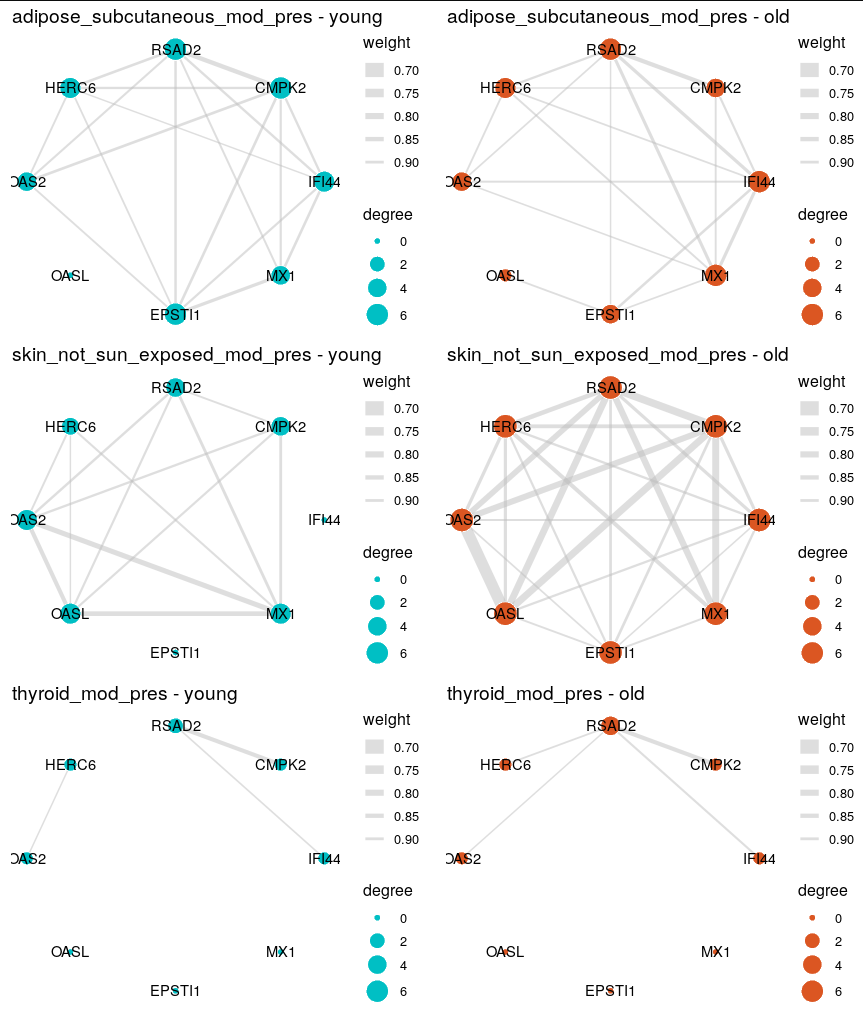
\includegraphics[width=1\textwidth]{img/chap2/chap2_graphs_intersection_plot_adipo_skinnosun_thyr.png}
    \caption[Réseaux de co-expression des gènes de l'intersection associée au phénomène d'inflammation lors du vieillissement entre les deux tranches d'âge]{Réseaux de co-expression des gènes de l'intersection associée au phénomène d'inflammation lors du vieillissement entre les deux tranches d'âge. Le réseau est filtré à 0.95 de dissimilarité (sur une échelle de 0 à 1) pour des questions de lisibilité et 3 tissus sont présentés : tissu adipeux, peau non exposée au soleil et thyroïde.}
    \label{figure:graphs_intersection_plot_adipo_skinnosun_thyr}
\end{figure}


\subsection{Les variation de co-expression dans l'intersection liée à l'inflammation}

L'inflammation systémique chronique de faible intensité est une des marques connues du vieillissement \citeB{Lopez-Otin2013, Franchini2006}. La complexité des mécanismes d'immunité et d'inflammation rend ce phénomène particulièrement difficile à étudier et les publications actuelles tendent donc à cibler peu d'acteurs en même temps (gène, protéine, miARN, etc.) et à se concentrer sur des contextes très précis \citeB{Franceschi2017}. Bien qu'apportant un niveau de preuve inférieur à toute validation expérimentale, les réseaux de co-expression de gènes permettent de comprendre bien plus d'acteurs. À titre d'exemple, on a souhaité ici détailler le cas de l'intersection de gènes associés à l'inflammation lors du vieillissement (Figure \ref{figure:revigo_resume_4_enrich}.D).


Les variations de motif dans la co-expression sont bien souvent la première cause de non-préservation des modules \citeB{Ritchie2016}. Des changements de score de centralité, des modifications de gène pivot (\textit{hub gene}), des suppressions totales de signal sont bien souvent à l'origine de cette différence de topologie détectée entre les modules à l'aide de la co-expression différentielle \citeB{Ritchie2016,Zhang2005a}. Cet effet se manifeste de plusieurs façons dans le cas de l'intersection sur l'inflammation comme visible en figure \ref{figure:graphs_intersection_plot_adipo_skinnosun_thyr}. Bien que la variation de la co-expression ne soit pas identique entre tous les tissus qui forment cette intersection, on observe des acteurs communs. Le gène RSAD2 précédemment mis en avant comme gène simulé par le FT IRF1 et un mARN devient ainsi un gène pivot dans la condition âgée selon le classement de score de centralité. Cependant, les sources de progression dans le classement selon la centralité divergent selon le tissu. Dans le tissu adipeux on constate que c'est dû à un renfort de la co-expression entre RSAD2 et IF44 associé à une perte partielle de co-expression globale par CMPK2, gène pivot dans la condition jeune. Dans la peau non exposée au soleil, on constate un renfort global de la co-expression avec toutefois une centralisation vers RSAD2. Une augmentation localisée entre OAS2 et OASL est également à noter. Enfin, dans la thyroïde, c'est une déconnexion entre HERC6 et OAS2 au profit de RSAD2 qui le rend gène pivot dans la condition âgée. Si cette réorganisation de la co-expression vers RSAD2 aurait pu être issue d'une contribution d'IRF1 ou tout autre IRF étant donné les informations précédentes, des analyses complémentaires ont précisé qu'aucun des IRF détectés comme FT auparavant n'était présent dans le module où se trouve RSAD2 (jeune comme âgé). L'origine de la variation de RSAD2 et OAS2/OASL pourrait donc être d'une autre nature qu'une modification de la transcription d'un ou plusieurs FT.

\begin{figure}[p]
    \centering
    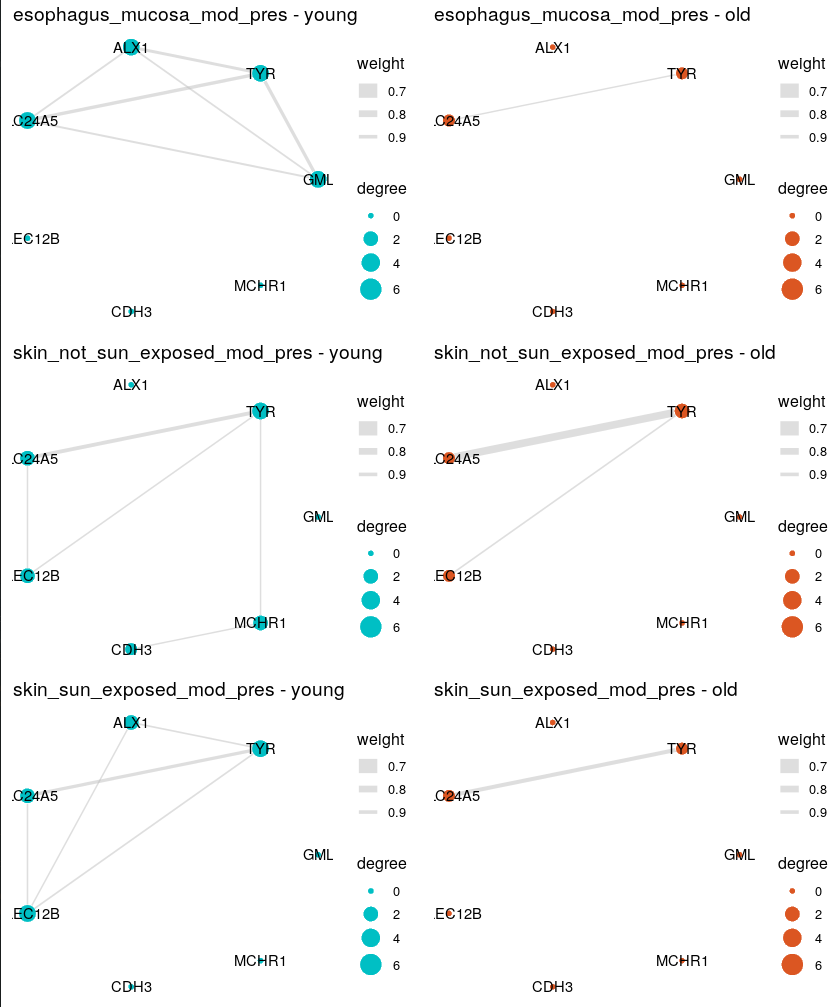
\includegraphics[width=1\textwidth]{img/chap2/chap2_graphs_intersection_melanine.png}
    \caption[Réseaux de co-expression des gènes de l'intersection associée à la surproduction de mélanine lors du vieillissement entre les deux tranches d'âge]{Réseaux de co-expression des gènes de l'intersection associée à la surproduction de mélanine lors du vieillissement entre les deux tranches d'âge. Le réseau est filtré à 0.99 de dissimilarité (sur une échelle de 0 à 1) pour des questions de lisibilité et 3 tissus sont présentés : muqueuse œsophagienne, peau non exposée au soleil et peau exposée au soleil.}
    \label{figure:graphs_intersection_melanine}
\end{figure}


\subsection{Cas particulier : le vieillissement spécifique à la peau}

Si le vieillissement partage des mécanismes et altérations communes à travers plusieurs tissus, il existe parallèlement des altérations spécifiques à certains tissus. Bien que ne permettant pas l'enrichissement global de la compréhension du vieillissement, ces altérations locales nécessitent de s'y intéresser afin de prévenir et prendre en charge les pathologies qui s'y rattachent. En étudiant les intersections ne présentant pas d'enrichissements liés aux mécanismes communs du vieillissement et en tenant compte des tissus inclus, on peut ainsi étudier l'impact du vieillissement spécifique du tissu.
% La peau est un des organes dont l'intégrité est la plus susceptible d'être mise à mal par le vieillissement en raison de son exposition directe avec l'environnement extérieur. 
% Le premier facteur de vieillissement extrinsèque est le photo-vieillissement dont les effets sont cumulatifs avec le temps \citeB{Farage2008}. Il se caractérise majoritairement pas une exposition aux UVs (UVA et UVB) qui vont induire des détériorations des fibres de collagène et d'élastine dans la peau. À noter également, des altérations de la matrice extra-cellulaire entre l'épiderme et le derme qui sont les deux couches composant la peau \citeB{Rogowski-Tylman2016}. 

% Une intersection faite de la peau exposée au soleil, la peau non exposée au soleil et la muqueuse œsophagienne fait état dans notre cas d'un tel type de photo-vieillissement. 
Une intersection faite de la peau exposée au soleil, la peau non exposée au soleil et la muqueuse œsophagienne fait état dans notre cas d'un tel type de vieillissement. 
Elle est en effet composée principalement d'enrichissements sur des fonctions physiologiques directement liées à la synthèse et régulation de mélanine comme exposé en Figure \ref{figure:revigo_resume_melanine}.
% Ce pigment synthétisé par les mélanocytes à partir d'une oxydation de la tyrosine joue un rôle majeur de lutte contre les dégâts provoqués par les UV \citeB{Bettley1965}. 
C'est le gène TYR, impliqué dans cette synthèse qu'on trouve dans le réseau de co-expression de notre intersection qui entraîne notamment cet enrichissement. Il est détecté comme gène pivot (score de centralité) dans chacun des tissus et chacune des tranches d'âge (Figure \ref{figure:graphs_intersection_melanine}), attestant ainsi de son rôle majeur dans la régulation de la mélanogénèse. On constate qu'il est lié dans la condition jeune par une relation forte (dissimilarité < 0.8 en moyenne) avec un autre gène, SLC24A5. Ce gène est connu pour coder pour un échangeur de cations (sodium, potassium, calcium) de façon générale et a été plusieurs fois soupçonné d'une contribution à la régulation de la mélanogénèse \citeB{Zhang2019,Ginger2008}. C'est notamment à lui que se rattachent les enrichissements de type \textit{secondary metabolite biosynthetic process}. 
% Aucune confirmation de son rôle de régulateur partiel de la production de mélanine n'a été faite chez l'homme malgré sa mise en évidence chez la souris . 
% Contrairement à la tyrosinase produite par TYR qui se trouve dans les mélanosomes, la protéine NCKX5 produite par SLC24A5 est localisée dans les mitochondries. 
% dans le cas des deux tissus de peau, mais pas dans la muqueuse œsophagienne
À ces deux gènes s'ajoute une relation de chacun avec CLEC12B dans le cas des deux tissus de peau et pas de la muqueuse œsophagienne. Ce gène appartient à la famille des récepteurs de lectine de type C qui jouent un rôle essentiel dans l'immunité et l'homéostasie à laquelle contribue la mélanine localement. La fonction de CLEC12B elle-même reste cependant encore mal caractérisée malgré la présence d'un motif d'inhibition basé sur la tyrosine d'un immunorécepteur dans son domaine intracellulaire. Ceci lui permettrait donc de recruter SHP-1/SHP-2 \citeB{Hoffmann2007Aug, Tone2019}, deux phosphatases suspectées d'avoir un rôle dans la progression des mélanomes \citeB{Zhang2013}. 

\begin{figure}[hb]
    \centering
    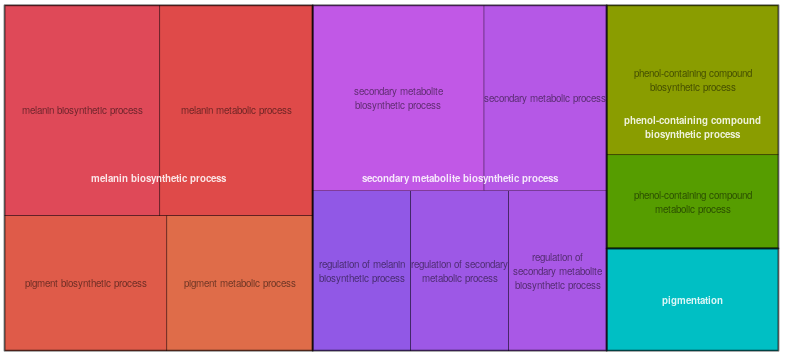
\includegraphics[width=1\textwidth]{img/chap2/chap2_revigo_resume_enrich_skin.png}
    \caption[Résumé des enrichissements sur GO par carte proportionnelle de l'intersection peau exposée au soleil, peau non exposée au soleil et muqueuse œsophagienne]{Résumé des enrichissements sur GO par carte proportionnelle de l'intersection peau exposée au soleil, peau non exposée au soleil et muqueuse œsophagienne. Chaque ensemble de GO terme partageant une ontologie parente commune (selon un score de similarité) est groupé sous une même couleur.}
    \label{figure:revigo_resume_melanine}
\end{figure}

La Figure \ref{figure:graphs_intersection_melanine} permet de constater que la relation TYR/SLC24A5 tend à augmenter avec l'âge dans la peau exposée ou non au soleil. Si l'augmentation est très marquée la peau non exposée au soleil, elle est bien moindre dans la peau non exposée. Ces résultats coïncident avec l'augmentation de la production de mélanine constatée chez la personne âgée pour compenser la diminution globale de la densité de mélanocytes \citeB{Gilchrest1979}. À l'inverse, la co-expression de CLEC12B avec SLC24A5 et TYR tend à diminuer avec l'âge, ainsi que l'intégralité de la co-expression de l'intersection.

La muqueuse œsophagienne elle semble interagir plus étroitement avec deux autres gènes, GML et ALX1 avec toutefois une interaction notable de la peau exposée au soleil avec ALX1 également. ALX1 est un gène jouant un rôle dans la migration cellulaire dans les structures craniofaciale lors du stade embryon, tandis que la fonction de GML est peu connu en dehors d'une potentielle contribution dans la voie d'activation de l'apoptose via p53 en cas de dommage à l'ADN. Comme visible en Figure \ref{figure:graphs_intersection_melanine}, la relation entre ces gènes ainsi qu'avec le gène TYR tend à diminuer dans la tranche âgée, qu'il s'agisse de la muqueuse œsophagienne comme de la peau exposée au soleil.




\section{Discussion}

\subsection{La susceptibilité des tissus aux variations liées au vieillissement}

Le vieillissement peut être vu comme une imbrication de multiples phénomènes qui découlent d'une dérégulation du fonctionnement physiologique ou d'une réponse à cette dérégulation. En prenant en compte le système dans sa quasi-intégralité, les réseaux de co-expression permettent d'acquérir de nouvelles connaissances au-delà d'acteurs transcriptomiques individuels connus. Les variations au cours du temps des relations de co-expression entre gènes sont alors les témoins d'autant de voies d'activations qui s'altèrent. Leur suivi et mise en contraste au travers de la co-expression différentielle sont donc à leur tour un moyen supplémentaire de comprendre le déroulé des altérations \citeB{Sharan2006, Southworth2009}. En comparant ces dernières entre de multiples tissus, il est possible d'en déduire des mécanismes communs au vieillissement, et à l'inverse ceux spécifiques. Dans cette étude, on s'est donc attachés à étudier ce vieillissement d'un point de vue multi-dimensionnel en comparant les réseaux issus de multiples tissus, et ce, entre deux tranches d'âge extrêmes. 

Si le vieillissement tend à perturber de nombreuses fonctions physiologiques, il semble cependant que peu de gènes soient impactés ou impactant dans ce processus. Ainsi, comme cela a pu être observé auparavant \citeB{Avelar2019}, une minorité de gènes varie significativement entre les deux conditions (modules NP) et une proportion légèrement plus grande varie modérément (modules MP) (Figure \ref{figure:upset_intersection_genes_tissu_unpres_modpres}). Ces gènes suffisent pourtant à représenter une large majorité des phénomènes connus du vieillissement : perte d'homéostasie, instabilité génomique, inflammation, dérivés réactifs de l'oxygène, etc. (Table \ref{table:intersection_aging_global_phenomenons} et Figure \ref{figure:revigo_resume_4_enrich}). Si leur répartition est inégale entre les tissus, ceux en portant le plus coïncident avec les tissus ayant un fort taux de renouvellement \citeB{Armanios2012, Barker2010, Leblond1956} (Table \ref{table:intersection_aging_global_phenomenons}) à l'exception dans notre cas de la thyroïde dont le renouvellement cellulaire minimal est de 8 ans \citeB{Coclet1989Dec}. Malgré une évidence des modifications que subit le système endocrinien avec le vieillissement, l'impact de celui-ci sur la thyroïde reste peu documenté hors pathologies graves \citeB{Faggiano2011Sep}. En effet, les altérations endocrines thyroïdiennes (hypo ou hyperthyroïdies) sont souvent associées à un vieillissement "naturel" de la personne \citeB{Cooper2004Dec}. Il est donc présomptueux ici de s'essayer à trouver une cause d'autant de marques du vieillissement sans plus d'information. Pourtant, les indices d'un rôle de la thyroïde sur la longévité s'accumulent ces dernières années \citeB{Garasto2017Jul,Arosio2020Sep}. Renforcer les connaissances sur les altérations de la fonction thyroïdienne chez la personne âgée semble donc une voie intéressante pour l'amélioration de la durée de vie chez l'homme.


\subsection{La variation de la réponse inflammatoire issue du vieillissement}

L'inflammation chronique de faible intensité est une caractéristique majeure du vieillissement qu'on nomme en anglais "\textit{inflammaging}" \citeB{Franceschi2014Jun,Minciullo2015} et dont la complexité limite encore les connaissances à son sujet \citeB{Franceschi2017}. Si l'inflammation est un mécanisme bénéfique dans la réponse aigüe et temporaire à un pathogène, elle se retrouve délétère dans le cas du vieillissement malgré une faible intensité car elle est persistante. Ce phénomène assumé comme étant un précurseur de plusieurs autres phénomènes du vieillissement \citeB{Lopez-Otin2013} s'est retrouvé ici plutôt exprimé dans le tissu adipeux, la peau non exposée au soleil, ainsi que la thyroïde. Les enrichissements fonctionnels sont venu préciser cette composante de l'inflammation comme une réponse à une réaction virale. En cause, de nombreux régulateurs d'interférons de type I significativement enrichis malgré leur absence de l'intersection. Ceci s'explique à contrario par la présence de nombreux gènes de réponse aux interférons, stimulés en temps normal par la présence d'ARN ou ADN viral.

Les interférons de type I (IFN-I) sont des cytokines regroupant tous les interférons à l'exception des IFN-\textgamma{} et dont les interférons majoritaires sont les IFN-\textalpha{} et IFN-\textbeta{}. Ces IFN-I ont pour rôle, dans la réponse inflammatoire normale, d'entraver à la fois la réplication du virus et les cellules hôtes infectées. Pour cela, un large panel de gènes de réponse aux interférons, dont ceux détectés ici, est induit avec différents objectifs : interférer avec le trafic intracellulaire des vésicules, limiter la stabilité et la traduction des ARNm viraux, et entraîner une apoptose de la cellule au besoin via la voie d'activation de la protéine p53\citeB{Frisch2020}. Cependant l'intervention de ce mécanisme antiviral dans le cadre du vieillissement est encore mal compris. Une hypothèse prometteuse est que des éléments transposables, plus particulièrement les LINE-1 (\textit{long interspersed nuclear elements}) se retrouvent non réprimés avec l'âge en raison d'une dégradation des acteurs de leur répression (ex : des petits ARN ou \textit{small RNA} (smRNA) en anglais) \citeB{Kreiling2017Jan, DeCecco2019Feb, Frisch2020}. Ces LINE-1 codent alors pour diverses transcriptases inverses et autres protéines de rétro-transposition qui vont déclencher la réponse anti-virale associée à une sénescence \citeB{QiujingYu2015May}. S'il est admis que cette réponse varie de la "normale" antivirale, il reste toutefois difficile de comprendre comment les gènes antiviraux se comportent dans ce cadre non-viral \citeB{Frisch2020} et la raison pour laquelle des marqueurs de la sénescence sont produits.

Dans le cadre de notre étude, on a constaté que le gène antiviral RSAD2 induit par les interférons officie comme gène pivot de co-expression. Dans le cas de la peau non exposée au soleil, il collabore également étroitement avec deux autres gènes antiviraux de la famille OAS : OAS2 et OASL. Les gènes OAS ont déjà été auparavant associés à une réponse de type IFN-I induite par la sénescence et plus particulièrement l'accumulation d'ADN dans la cellule \citeB{DeCecco2019Feb} qui est une composante délétère du vieillissement. Concernant RSAD2, aucun lien direct chez l'humain n'a été mis en avant à ce jour, seulement chez la souris \citeB{Ma2020Mar}. La protéine produite par RSAD2 est connue pour limiter la réplication de l'ADN viral ou de l'ARN double brin viral bien que le mécanisme par lequel elle opère n'est pas entièrement clair \citeB{Fitzgerald2011Jan}. En plus d'être un potentiel marqueur de cette accumulation d'ADN liée aux éléments transposables, RSAD2 pourrait donc être un potentiel gène candidat pour le développement de médicaments anti-âge.


\subsection{L'altération de la régulation des mélanocytes et de la mélanogénèse avec l'âge}

Au-delà des manifestations communes du vieillissement, chaque tissu est affecté de façon plus spécifique dans sa physiologie. L'altération avec l'âge de la mélanogénèse est un de ces changements qu'on retrouve en toute logique uniquement dans les tissus disposant de mélanocytes. La peau est l'organe en disposant du plus grand nombre et se retrouve ainsi d'autant plus affecté par cette altération avec l'âge. Dans notre intersection liée à la mélanogénèse, l'hyper-pigmentation connue dans le vieillissement \citeB{Hakozaki2016Sep} s'est retranscrite par l'augmentation de la co-expression entre TYR et SLC24A5, respectivement catalyseur et régulateurs de la production d'eumélanine \citeB{Cullinane2011Oct, Ginger2008}, dans la peau exposée ou non au soleil. L'augmentation nettement plus grande dans la peau non exposée au soleil était toutefois inattendue étant donné que l'hyper-pigmentation a plutôt été relevée dans les peaux exposées au soleil en raison de la stimulation de la mélanogénèse par les UV \citeB{Gilchrest1979}. 

En plus d'une co-expression entre TYR et SLC24A5, une forte co-expression de CLEC12B a été montrée dans les deux tissus de peau. Une investigation de ce gène a révélé que peu d'information est connue sur ses fonctions et son implication dans la mélanogénèse. Des résultats préliminaires conséquents ont toutefois montré sa capacité à recruter les phosphorylases SHP-1/SHP-2 via son domaine ITIM \citeB{Sormani2019}, enzymes notamment connues pour leur implication dans la pigmentation dans le syndrome LEOPARD \citeB{Motegi2015}. Ce nouveau gène impliqué dans la pigmentation de la peau coïncide ainsi avec les estimations d'un plus grand nombre de gènes contribuant au spectre de pigmentation que ceux actuellement connus et majeurs comme MC1R \citeB{Parra2004Nov}. 
Contrairement à la co-expression entre TYR et SLC24A5, CLEC12B tend à perdre sa synergie avec l'âge. Avec l'âge, CLEC12B tend à perdre sa synergie avec TYR et SLC24A5. L'inactivation de CLEC12B ayant démontré une diminution de la pigmentation dans un modèle de peau humaine reconstruite \citeB{Sormani2019}, on peut alors se demander si ce gène ne serait pas impliqué dans le phénomène de dépigmentation global de la peau lors du vieillissement (phénomène parallèle à l'hyper-pigmentation locale). Plus précisément, CLEC12B serait impliqué dans les voies d'inhibition de la prolifération des mélanocytaire par le biais de p53/p21/p27 \citeB{montaudie2019} et on pourrait envisager alors que la diminution de la densité de mélanocytes avec l'âge serait en partie dû à la diminution de co-expression de CLEC12B avec TYR et SLC24A5. Une validation expérimentale par une limitation partielle de l'expression de CLEC12B pourrait être à même de confirmer cette hypothèse.

La muqueuse œsophagienne et la peau étant toutes deux des tissus dotés d'un épithélium squameux stratifié dérivé de la crête neurale \citeB{delaPava1963}, il est cohérent de les retrouver au sein d'une même intersection. Pierson et al. ont d'ailleurs montré la proximité de leur expression dans leur étude du jeu de données GTEx \citeB{Pierson2015}. S'il est commun que la peau soit étudiée pour son contenu en mélanocytes, il est beaucoup moins courant que le contenu en mélanocytes de la muqueuse œsophagienne soit étudié. Le rôle de ce type cellulaire dans ce tissu reste ainsi encore mal compris en dehors des parallèles avec les mécanismes déjà connus dans la peau comme la réduction des dérivés réactifs de l'oxygène ou la fixation de certaines molécules organiques et ions métalliques \citeB{Tolleson2005}. 

Dans cette intersection côté muqueuse œsophagienne donc, la co-expression de TYR et SLC24A5 avec CLEC12B fait place à une co-expression croisée de TYR et SLC24A45A avec ALX1 et GML. 
GML est un homologue des protéines de membrane ancrées de type glycosyl-phosphatidylinositol (GPI), mais dont la fonction encore inconnue est suspectée d'être liée à l'apoptose et la régulation du cycle cellulaire \citeB{Furuhata1996Nov}. Il a été constaté que son expression tend à ralentir la progression des cellules cancéreuses de l'œsophage et à augmenter la sensibilité des cellules cancéreuses à certaines chimiothérapies \citeB{Catalano2001May}. 
De son côté, ALX1 est un facteur de transcription impliqué dans la régulation de gènes liés au développement embryonnaire et à la migration cellulaire \citeB{Dee2013Jan}. Il a été détecté comme sous exprimé chez des embryons de souris irradié entraînant un retard de pigmentation de l'épithélium rétinien. 
Pris ensemble, ces gènes pourraient donc être soupçonnés d'être à l'origine de la régulation de la prolifération des mélanocytes dans la muqueuse œsophagienne, bien qu'aucune direction de régulation ne puisse être extrapolée de nos réseaux de co-expression en tant que tel. En revanche, on peut avancer que si une telle régulation existe, elle est perturbée avec le vieillissement d'après la diminution notable de la co-expression entre TYR et SLC24A5 (donc contraire à l'évolution de la co-expression dans la peau) coïncidant avec la forte diminution de leur co-expression avec ALX1 et GML ainsi qu'entre eux deux. 
Ces altérations et les fonctions pour lesquelles codent ces gènes évoquent logiquement le développement de mélanomes qui sont parmi les pathologies associées au vieillissement et où les fonctions de régulation de la prolifération des mélanocytes par ALX1 et GML pourraient entrer en jeu. Toutefois, le mélanome œsophagien reste une pathologie rare, même si la fréquence des mélanomes œsophagiens d'origine métastatique est plus élevée que celle des mélanomes œsophagiens d'origine primitive. Il reste donc compliqué d'évaluer l'impact de la diminution de co-expression de ALX1 et GML ainsi que SLC24A5 et TYR dans le vieillissement de la muqueuse œsophagienne. Si des études sont menées ultérieurement sur ces gènes ou sur le contenu en mélanocytes de la muqueuse œsophagienne, elles pourront potentiellement donner de nouvelles perspectives à ces résultats.





\section{Conclusion}

Grâce à leur capacité d'étude à plus large échelle, les réseaux de co-expression sont un outil à privilégier pour l'exploration multi-tissus d'un phénomène aussi global et complexe que le vieillissement. Notre mise en évidence de groupes gènes impliqués dans les deux phénomènes du vieillissement sur lesquels on s'est concentrés est encourageant quant à l'utilisation de la co-expression différentielle et l'étude des motifs impliqués. Des tissus portant les mêmes gènes d'altérés peuvent ainsi être étudiées via la co-expression et permettre d'établir un lien direct entre les gènes et les marques du vieillissement. Des phénomènes communs comme spécifiques de différents tissus ont pu être mis en évidence. Des limitations restent toutefois présentes sur la nécessité pour se faire d'un grand nombre d'échantillons dans les tranches d'âge jeunes, ou en tout cas pas sur tout type de tissu. 
% De même, une validation de ces résultats via expérimentalement reste un passage obligatoire et coûteux, bien que moins coûteux qu'un criblage à haut débit sans pré-sélection.
De même, une validation de ces résultats via expérimentalement reste un passage obligatoire et coûteux. Notre profilage par co-expression différentielle aura toutefois permis de réduire leur coût financier en ciblant un sous ensemble de gènes à étudier par rapport à un criblage à haut débit sans pré-sélection.





% ##############################################################################

% Idées initiales de chapitre 2 - abandonnées :
% \begin{itemize}
%     \item Rajout d'information protéique pour "consolider" le réseau ?
%     \item Rajout d'une méthode de réseau consensus à GWENA ?
%     \item Differential co-expression avec un autre tissu sur lequel on peut avoir des jeux de données jeune/vieux pour récup les genes communs au vieillissement, ceux specifique à un tissu ou l'autres, et ceu combinant le vieillissement specifique au tissu ?
%     \item Une étude de l'impacte de la filtration sur l'état du réseau final ? Il n'y a rien de systemique dans la littérature, personne qui en fasse une review. Parsana et al. (alexis battle team) a fait ça en 2019 pour tester la PC-correction uniquement. Ils ont simulé des données scale free + des données scale free mimiquant GTEx et essayé de déterminer l'impact en calculant un FDR
% \end{itemize}


\bibliographystyleB{unsrt}
\bibliographyB{chap2-biblio}
% \bibliographystyleB{plain-fr}
% \bibliographyB{bibliographie}